\documentclass[10pt,twocolumn,letterpaper]{article}

\usepackage{iccv}
\usepackage{times}
\usepackage{epsfig}
\usepackage{graphicx}
\usepackage{amsmath}
\usepackage{amssymb}

%%%%% 
\usepackage{subfigure}
\usepackage{multirow}
\usepackage{amsthm,mathrsfs,amsfonts,dsfont}
\usepackage{algorithm}
\usepackage{algorithmic}
\renewcommand{\algorithmicrequire}{\textbf{Input:}}
\renewcommand{\algorithmicensure}{\textbf{Output:}}
\usepackage{epstopdf}
\usepackage{bm}
\newtheorem{corollary}{Corollary}
\newtheorem{definition}{Definition}
\newtheorem{theorem}{Theorem}
\newtheorem{proposition}{Proposition}
\newtheorem{lemma}{Lemma}
\newtheorem{remark}{Remark}


\def\M{\mathcal{M}}
\def\R{{\mathbb R}}
\def\bR{{\bf R}}
\def\U{{\bf U}}
\def\V{{\bf V}}
\def\diag{\mbox{diag}}
\def\bsigma{\mbox{{\boldmath $\sigma$}}}
\def\trsp{{\sf T}}
\def\I{{\bf I}}
\def\0{{\bf 0}}
\def\G{{\bf G}}
\def\grad{{\text{grad}}}
\def\bZ{{\bf Z}}
\def\bfeta{\mbox{{\boldmath $\eta$}}}
\def\mT{{\mathcal T}}

\def\bB{{\bf B}}
\def\bN{{\bf N}}
\def\bM{{\bf M}}
\def\bD{{\bf D}}
\def\bI{{\bf I}}
\def\bE{{\bf E}}
\def\blambda{{\bm \lambda}}
\def\calL{{\mathcal{L}}}
\def\calC{{\mathcal{C}}}
\def\calS{{\mathcal{S}}}
\def\calF{{\mathcal{F}}}
\def\bL{{\bf L}}
\def\bO{{\bf O}}
\def\bU{{\bf U}}
\def\bV{{\bf V}}
\def\dsR{\mathds{R}}
\def\bX{{\bf X}}
\def\bx{{\bf x}}
\def\btx{{\tilde{\bf x}}}
\def\by{{\bf y}}
\def\bw{{\bf w}}
\def\btw{{\tilde{\bf w}}}
\def\tK{\tilde{K}}
\def\txi{\tilde{\xi}}
\def\tildeb{{\tilde{b}}}
\def\tphi{{\tilde{\phi}}}
\def\bz{{\bf z}}
\def\br{{\bf r}}
\def\bv{{\bf v}}
\def\bb{{\bf b}}
\def\bp{{\bf p}}
\def\bA{{\bf A}}
\def\bI{{\bf I}}

\def\bx{{\bf x}}
\def\bX{{\bf X}}
\def\by{{\bf y}}
\def\bY{{\bf Y}}
\def\bw{{\bf w}}
\def\bW{{\bf W}}
\def\balpha{{\bm \alpha}}
\def\bmu{{\bm \mu}}
\def\bK{{\bf K}}
\def\bg{{\bf g}}
\def\bp{{\bf p}}
\def\p{p}
\def\bP{{\bf P}}

\def\balpha{{\bm \alpha}}
\def\bbeta{{\bm \beta}}
\def\eg{{\emph{e.g.}}}
\def\zerocolumn{{\bf 0}}

\def\ttTP{{\tt TP}}
\def\ttFP{{\tt FP}}
\def\ttFN{{\tt FN}}

\def\st{{\text{s.t.}}}
\def\etc{\emph{etc}}
\def\wrt{\emph{w.r.t}}
\def\ie{\emph{ie}}
\def\eg{\emph{eg}}
\def\rank{{\text{rank}}}
\def\Tr{{\text{Tr}}}

\def\yanred{\textcolor{red}}
\def\yanblue{\textcolor{blue}}
%%%%%

% Include other packages here, before hyperref.

% If you comment hyperref and then uncomment it, you should delete
% egpaper.aux before re-running latex.  (Or just hit 'q' on the first latex
% run, let it finish, and you should be clear).
\usepackage[pagebackref=true,breaklinks=true,letterpaper=true,colorlinks,bookmarks=false]{hyperref}

% \iccvfinalcopy % *** Uncomment this line for the final submission

\def\iccvPaperID{283} % *** Enter the ICCV Paper ID here
\def\httilde{\mbox{\tt\raisebox{-.5ex}{\symbol{126}}}}

% Pages are numbered in submission mode, and unnumbered in camera-ready
\ificcvfinal\pagestyle{empty}\fi
\begin{document}

%%%%%%%%% TITLE
\title{Late Fusion via Subspace Search with Consistency Preservation}

\author{First Author\\
Institution1\\
Institution1 address\\
{\tt\small firstauthor@i1.org}
% For a paper whose authors are all at the same institution,
% omit the following lines up until the closing ``}''.
% Additional authors and addresses can be added with ``\and'',
% just like the second author.
% To save space, use either the email address or home page, not both
\and
Second Author\\
Institution2\\
First line of institution2 address\\
{\tt\small secondauthor@i2.org}
}

\maketitle
%\thispagestyle{empty}


\begin{abstract}
In many real-world applications, data can be represented in multiple ways or multi-view features,
in order to describe various characteristics of data.
In this way, it could often improve the prediction performance by taking advantage of these feature together.
Late fusion, which combines the predictions of multiple features, is a commonly used approach to make the final decision for a test instance.
However, it is ubiquitous that different features would dispute on the data, which results in performance degeneration.
Therefore, there is a requirement of outlier rejection while preserving consistency among different classifier results.
In this paper, we propose an efficient matrix factorization based approach to fuse predictions from multiple sources,
which could avoid the performance degeneration caused by the controversy of multiple features on test data.
Extensive experiments demonstrate that the proposed method is effective to remove outliers and improve fusion performance.

\end{abstract}

\section{Introduction}


%背景 多model融合
Feature representation of objects, which transforms raw data into numerical features, is a prerequisite for most real-world applications.
There are often multiple ways to generate numerical features from raw data for visual recognition.
For example, for image data, one can construct hand-crafted features such as scale-invariant feature transform
(SIFT) feature~\cite{loweijcv2004distinctive} and Histograms of Gradients (HOG) feature~\cite{dalalcvpr2005histograms},
or extract features based on well-trained convolutional neural networks (CNNs)~\cite{krizhevsky2012imagenet}.
Moreover, text data can be represented by term frequency–inverse document frequency (tf-idf)~\cite{manning2008introduction} and word2vec~\cite{mikoloviclr2013efficient}.
Each category of features tends to capture some specific characteristics of data,
such as textures of images and frequencies of text data.
When building a prediction model, the model trained on one kind of feautures could be biased and hence may incur unsatisfactory performance.
Existing works have investigated the performance improvement by combining multiple kinds of features in real-world applications~\cite{gehler2009feature,ye2012robust,xuiccv2013feature,lai2015learning}.


%% late fusion is a common sigle model -> single feature, 介绍late fusion
Late fusion, a typical approach to obtaining the final decision on testing data, aims to fuse the predictions from different features.
A commonly used method is to learn weights for predictions from various features to combine them, which has a number of variations~\cite{gehler2009feature,xuiccv2013feature,lai2015learning}.
Among these algorithms, multiple kernel learning (MKL)~\cite{lanckriet2004learning,Rakotomamonjy2008Simplemkl} is often used to train such a weighted combination.
However, a single feature may produce corrupted predictions on some data, which likely degenerates performance.
To deal with this issue, therefore, some works formulate it as a robust low-rank matrix recovery problem~\cite{gaoijcai2016robust,ye2012robust} by nuclear norm minimization.
Nevertheless, nuclear norm minimization applied in these works requires singular value decompositions (SVDs), which would be computationally unaffordable for large matrices.

\begin{figure}[!t]
\begin{center}
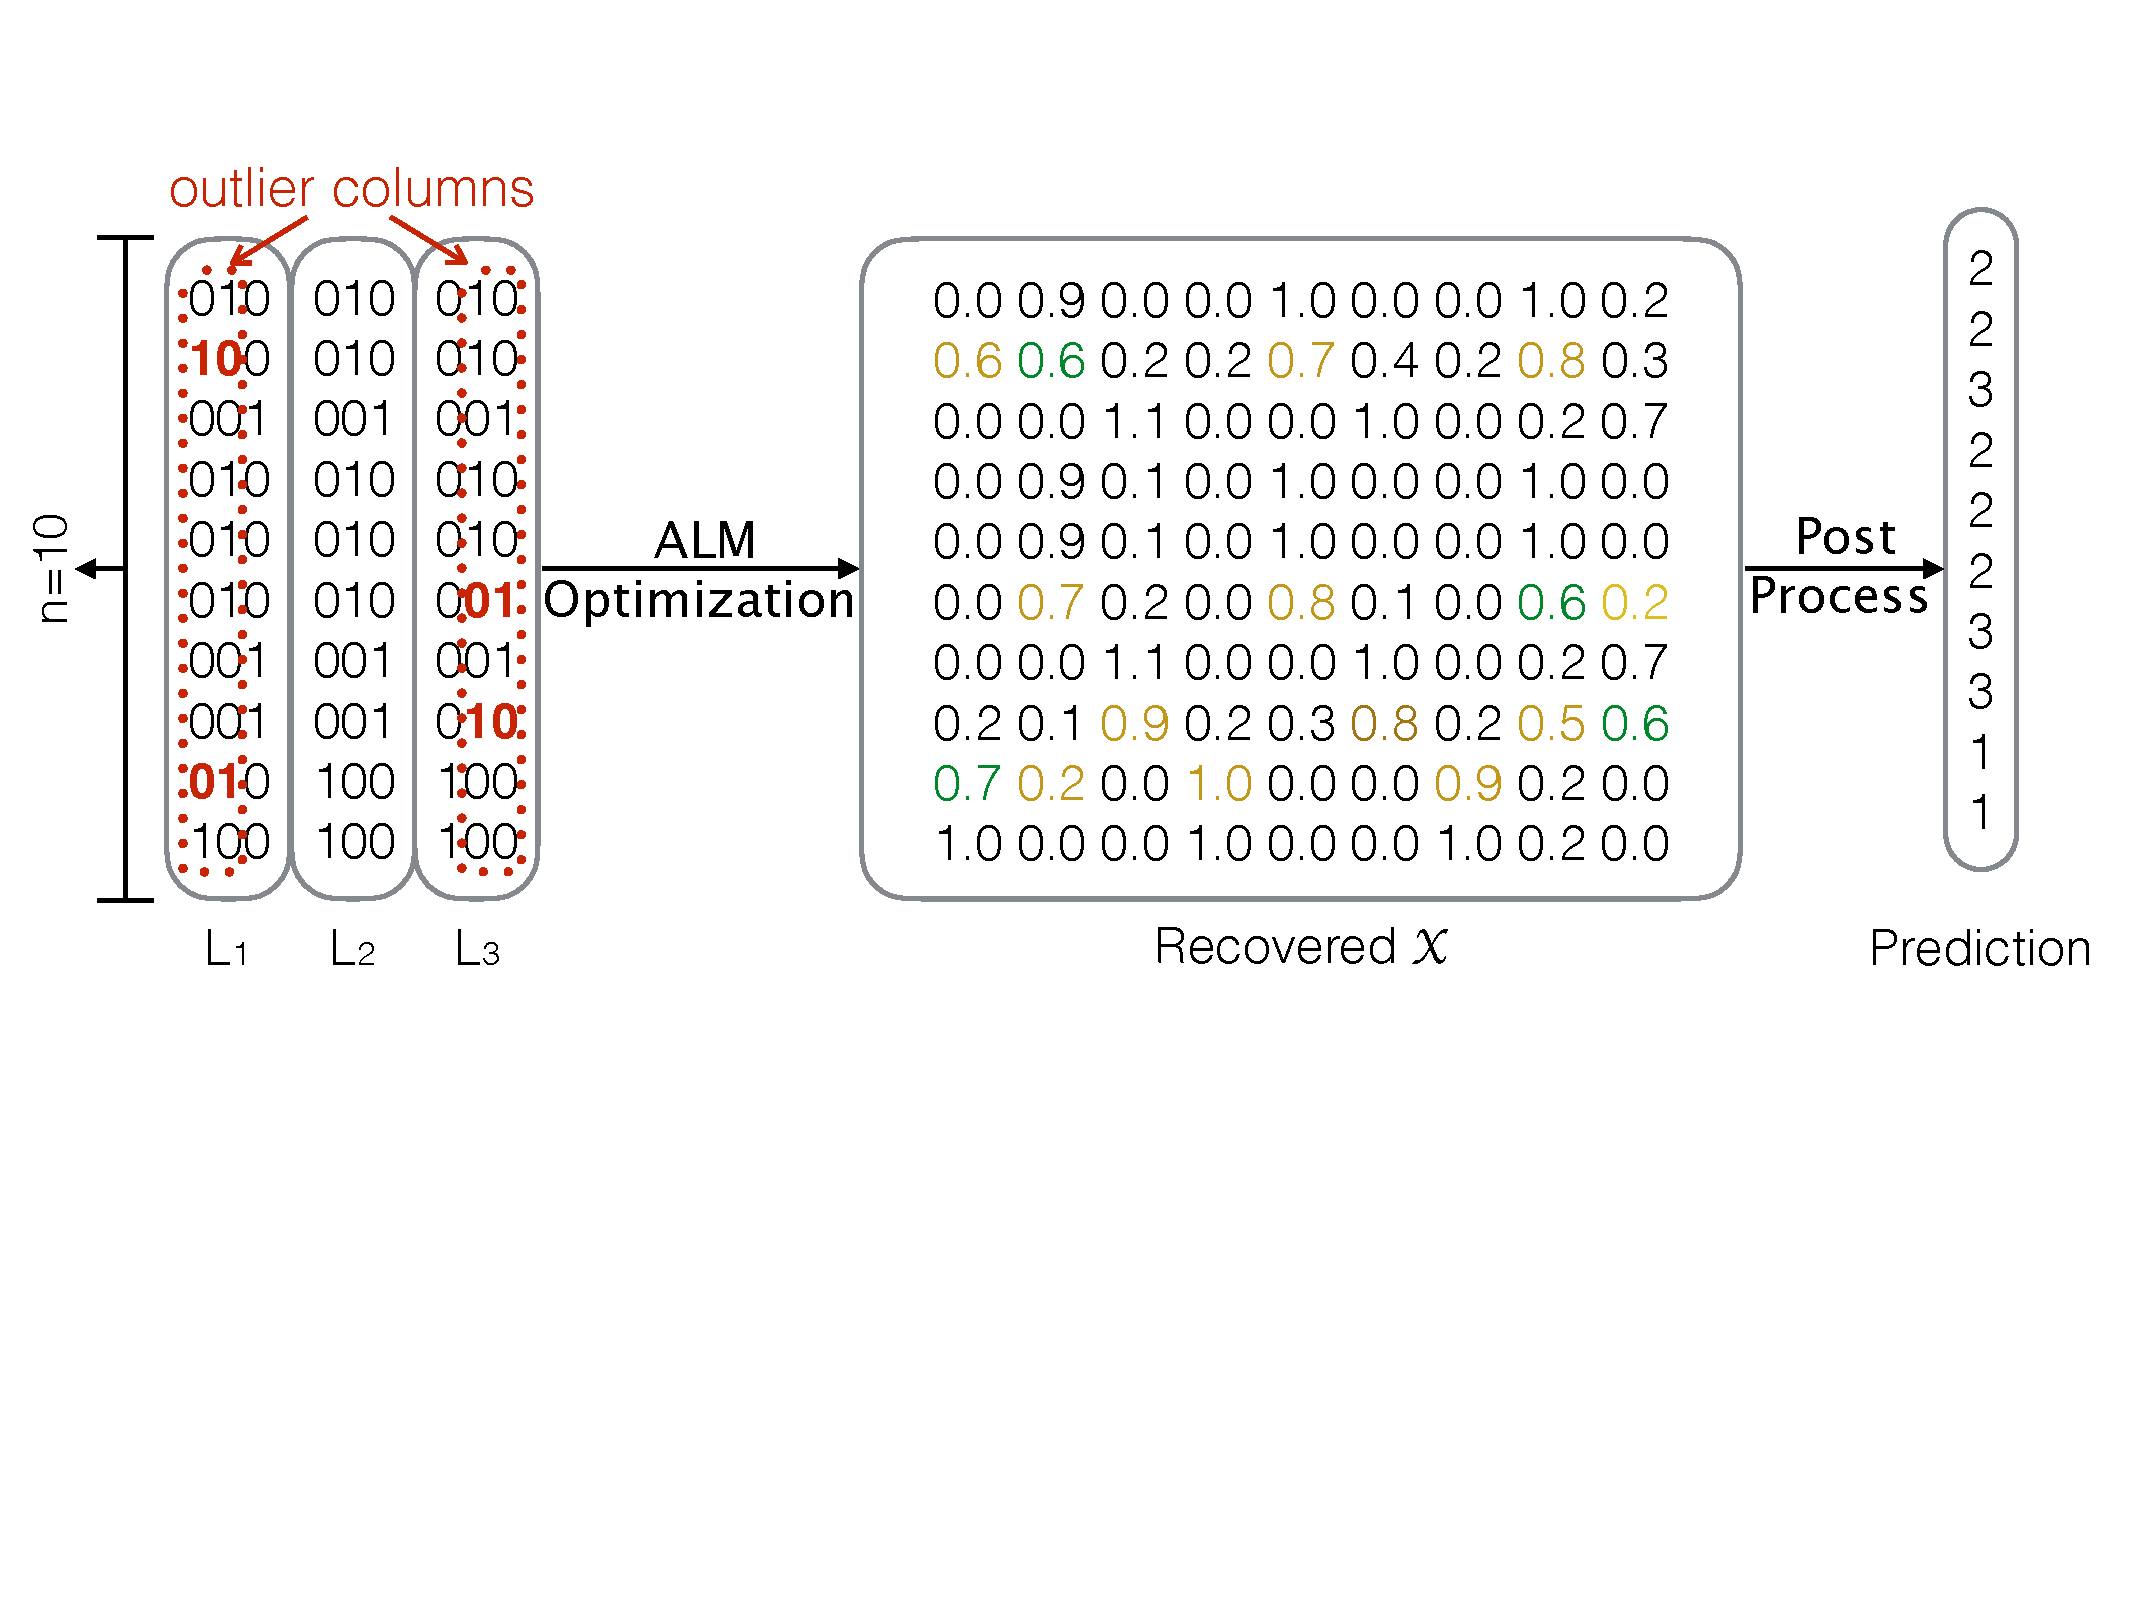
\includegraphics[width=0.48\textwidth]{resource/frame_work.pdf}
\end{center}
\caption{Framework of our late fusion algorithm.
In this example, there are 10 instances 3 classifiers and 3 classes.
Predictions of each classifier are converted to a binary indicator matrix,
denoted by $L_1$, $L_2$ and $L_3$.
Let $L = [L_1, L_2, L_3]$ be the label matrix.
Our algorithm detects and removes the outliers on $L$ and then recover the underlying low-rank subspace of $L$ as the prediction for testing instances.
We finally apply a post-processing method to generate the fused results.
%First, there are $\calC=3$ classifiers' results for $n=10$ instances.
%Each of them are converted into ``binary'' indicators from the soft prediction results, as $L = [L_1, L_2, L_3]$.
%Then, our ALM-based optimization process the binary indicator matrix into a recovered matrix $X$,
%which can be treated as soft prediction scores for testing instances.
%Finally, the fused prediction results are generated by a post-processing method.
}
\label{fig:framework}
\end{figure}

To prevent from the expensive nuclear norm minimization,
in this paper, we propose a more efficient matrix factorization algorithm to recover the underlying low-rank label matrix.
Particularly, our method searches the solution in a low-rank subspace under a fixed-rank constraint.
As for outlier detection,
we propose to filter out these inconsistent predictions on specific classes of models (See Fig.\ref{fig:framework}.
Notations are introduced shortly.).
Due to the fact that the $\ell_{1,2}$ loss preserves the fidelity within each column by $L_2$ loss in the vertical direction and is robust to sparse errors across all the columns by $L_1$ loss in the horizontal direction,
we apply this robust $\ell_{1,2}$ loss to remove the outlier columns in the label indicator matrix.
Furthermore, most existing matrix factorization optimization methods only consider smooth loss functions, rather than the nonsmooth loss.
We thus in particular present an approach based on augmented Lagrangian multiplier (ALM) to extend matrix factorization methods to nonsmooth problems.

The main contributions of this work are summarized as below:
\begin{itemize}
  \item We formulate the late fusion problem as a fixed-rank robust matrix recovery problem based on matrix factorization, which intuitively preserves the consistency of predictions from different sources.
  \item We propose an ALM based algorithm to extend existing matrix factorization algorithms from smooth least square loss to nonsmooth $\ell_{1,2}$ loss. 
  %\item Our proposed algorithm is more efficient than most state-of-the-art late fusion methods.
  %It is capable of handling large scale problems.
  \item Empirical studies show significantly improvement of our proposed method compared to existing late fusion algorithms.
\end{itemize}

\section{Related Work}
%% Matrix factorization
%% Fusion Methods

MKL based method is a simple but efficient way to combine different features for multi-model fusion,
and many improved algorithms have been proposed by introducing more constraint, boosting methods and other optimization.
In~\cite{vedaldi2009multiple}, the authors use MKL to learn an optimal combination of exponential ${\chi}^2$ kernels capturing a different feature channel.
In~\cite{gehler2009feature}, boosting approaches are proposed to ensemble different features, which learns the correct weighting of multiple predicted confidence scores from different models.
In~\cite{natarajan2012multimodal}, the authors propose a two-step strategy employing MKL and late score fusion methods to combine diverse features, specifically on event detection tasks.
In~\cite{lai2015learning}, a sample specific late fusion based on graph Laplacian with RankSVM style constraints is proposed,
which learns sample specific fusion weights by diffusing the information from labeled samples to the unlabeled one.
In~\cite{xuiccv2013feature}, a optimization algorithm are proposed to combine diverse decision values,
which learns the weights, thresholding and smoothing parameters in a joint framework.
However, all these mkl based fusion methods or others only learn weights to combine different basic models, which do not consider the outlier rejection in the fusion process specifically.

%Our proposed late fusion algorithm is based on matrix factorization,
%which has attracted increasing attention recently.
Matrix factorization has attracted increasing attention recently.
Many manifold optimization algorithms on matrix factorization have been proposed by exploiting the manifold geometry in a subspace.
Based on manifold optimization, fixed-rank matrices are supposed to belong to a smooth matrix manifold~\cite{Absil2008OAMM,vandereycken2013lowrank}.
In~\cite{vandereycken2013lowrank}, the authors propose a low-rank geometric conjugate gradient (LRGeomCG) method.
In~\cite{rtrmc2011boumal}, first- and second-order Riemannian trust-region methods are applied to solve the low-rank matrix completion by exploiting the low-rank constraint.
In~\cite{Bonnabel2011}, a linear regression algorithm is proposed, where the parameter of this algorithm is a fixed-rank matrix based on the Riemannian manifold geometry.
In~\cite{Mishra2012}, the authors propose a quotient geometric matrix completion method.
The authors in~\cite{grouse2010Balzano} propose an online algorithm for tracking subspaces, Grassmannian rank-one update subspace estimation.
In~\cite{ngonips2012scaled}, a gradient methods based on scaled metric on the Grassmann manifold is proposed.
The authors in~\cite{Wen2012} propose a low-rank matrix fitting algorithm to solve large scale matrix completion problems by exploiting nonlinear successive over-relaxation.
In~\cite{RechtNIPS2011hogwild}, a lock-free approach to parallelizing stochastic gradient descent is proposed.
However, all these matrix factorization methods only consider the general least square loss, which cannot be directly applied to handle $\ell_{1,2}$ loss.

Some other fusion algorithms are propsed for specific tasks, which would be hard to extend to general problems.
In~\cite{zheng2015query}, the authors estimate a feature’s effectiveness in a query-adaptive manner for image retrieval problems,
and they combine the scores of multiple features weighted by their effectiveness.
In~\cite{zha2015exploiting}, they use fusion features scores of different CNN layers and encoded features impove the accuracy of action recognition.
In~\cite{feichtenhofer2016convolutional}, the authors explore a variety of fusion methods to combine spatial and temporal CNN models, significantly improving the performance of two-stream network~\cite{simonyan2014two}.
\cite{wangmodality} proposes a framework use high-dimensional Fisher Vector features from RGB, HHA and surface normal modalities to effectively achieve state-of-the-art scene classification performance.
\cite{Wang_Transformation,tapaswi2015movieqa,yaohighlight} use some simple strategies to choose specific weight for different scores from multiple features.


\section{The Proposed Approach}

We first elaborate the formulation of our proposed algorithm,
which regards the late fusion problem as a robust matrix recovery problem.
Then we present the details of using ALM extending matrix factorization to handle $\ell_{1,2}$ loss.
Finally we introduce our post-process strategy to convert the recovered label matrix to final predictions.

\subsection{Problem Formulation}

Suppose there are $n$ testing instances and $\calC$ classes.
We denote each instance as $x_i \in \dsR^{d}$ where $1 \leq i \leq n$.
Assume that we have already trained $m$ classifiers, \ie. $f_1, f_2, ... f_m$.
Then by applying each single classifier $f_j$ ($1 \leq j \leq m$) on the entire testing data, one can derive an indicator matrix $\bL_j \in \dsR^{n \times \calC}$, where $\bL_{j, ic} = 1$ if the $i$-th instance is assigned to the $c$ class, otherwise $\bL_{j, ic} = 0$ (as shown in Figure~\ref{fig:framework}).
Let $\bL = [ \bL_1, \bL_2, ..., \bL_m ]$.
%%On one hand, we aim to preserve the consistency among $m$ classifiers, so we introduce a rank-$m$ constraint on $\bL$.
On one hand, we aim to preserve the consistency among $m$ classifiers, so we introduce a rank constraint on $\bL$.
On the other hand, to catch the outlier columns, we apply robust $\ell_{1, 2}$ loss, which is computed by
{\small
\begin{align}
|| \bX ||_{1,2} = \sum_{j = 1}^{m\calC} \sqrt{ \sum_{i = 1}^{n} \bX_{ij}^2 }
\end{align}
}
\noindent
Thus, the proposed model can be written as below:
{\small
\begin{align}\label{eq:l12_rankconstraint}
  \min_{\bX} ~&~ || \bL - \bX ||_{1,2}~~~~~~\st~~\rank(\bX) = p
\end{align}
}
\noindent
where $\bX \in \dsR^{n \times m\calC}$ is the underlying low-rank label matrix to be recovered, $\rank(\bX)$ obtains the rank of $\bX$,
and $p$ is a scalar.
In our setting, to preserve the consistency among various classifiers, we set $p = \calC$.


It is difficult to optimize Problem~(\ref{eq:l12_rankconstraint}) directly due to the presence of the rank constraint.
We hence transform the original problem as a matrix factorization formulation as below:
{\small
\begin{align}\label{eq:l12_mf}
  \min_{\bX} ~&~ || \bL - \bX ||_{1,2}   \nonumber \\
         \st ~&~ \bX = \bU \bV,~\bU \in \dsR^{n \times p},~\bV \in \dsR^{p \times m\calC}  .
\end{align}
}
\noindent
Nevertheless, existing matrix factorization algorithms focus on smooth loss functions, rather than a nonsmooth $\ell_{1,2}$ loss function~\cite{tanicml2014riemannian,vandereycken2013lowrank,Wen2012,ngonips2012scaled,rtrmc2011boumal}.
In the following section, we present an ALM optimization framework to solve Problem~(\ref{eq:l12_mf}).


\begin{algorithm}[ht]

\begin{algorithmic}

\REQUIRE $\bL \in \dsR^{n \times m\calC}$, rank($\bX$) = $p$

\STATE Initialize $\rho > 1$, $t = 0$, $\blambda_{0} = 0$, $\bE_{0} = 0$, and $\mu_{0} > 0$.

\WHILE{$t = 0$ or $L_1(\bE_{t+1}-\bE_{t}) \geq \epsilon$}

  \WHILE{not converge}

    \STATE 1: Obtain $\bX_{t+1}$ by solving Problem~(\ref{eq:subproblem_wrt_X}).

    \STATE 2: Obtain $\bE_{t+1}$ by solving Problem~(\ref{eq:column_wise_soft_thresholding}).

  \ENDWHILE

  \STATE 3: $\blambda_{t+1} = \blambda_{t} + \mu_{t} (\bL - \bX_{t+1} - \bE_{t+1})$.

  \STATE 4: $\mu_{t+1} = \rho \mu_{t}$.

  \STATE 5: t = t + 1.

\ENDWHILE

\ENSURE $\bX \in \dsR^{n \times m\calC}$

\end{algorithmic}
\caption{The ALM algorithm for Problem~(\ref{eq:mf_l21_constrained})}
\label{alg:alm_mf}
\end{algorithm}


\subsection{Optimization Based on ALM}

Most existing matrix factorization optimization methods only consider smooth loss functions, rather than the nonsmooth $\ell_{1,2}$ loss used in Problem~(\ref{eq:l12_mf}).
In this section, we present an ALM based algorithm to optimize Problem~(\ref{eq:l12_mf}).



By introducing a new variable $\bE = \bL - \bX$, we can develop Problem~(\ref{eq:l12_mf}) as below:
{\small
\begin{align}\label{eq:mf_l21_constrained}
  \min_{\bE, \bX} ~&~ || \bE ||_{1,2}      \nonumber \\
  \st             ~&~ \bE = \bL - \bX  ,   \nonumber \\
                  ~&~ \bX = \bU \bV,~\bU \in \dsR^{n \times p},~\bV \in \dsR^{p \times m \calC}
\end{align}
}
\noindent 
The augmented Lagrangian function of Problem~(\ref{eq:l12_mf}) is constructed as below
{\small
\begin{align}\label{eq:lagrangian_l21}
  \calL (\bX, \bE, \blambda, \mu) = &~ || \bE ||_{1,2} + \langle \blambda, \bL - \bX - \bE \rangle      \nonumber \\
                                    & + \frac{\mu}{2} || \bL - \bX - \bE ||_F^2
\end{align}
}
\noindent
where $\bX = \bU \bV$, $\mu$ is a scalar,
and $\blambda \in \dsR^{n \times m\calC}$ are the Lagrangian multipliers.
Here $\langle \bA, \bB \rangle$ is the inner product of $\bA \in \dsR^{m \times n}$ and $\bB \in \dsR^{m \times n}$, and defined as $\langle \bA, \bB \rangle = \sum_{i=1}^{n} \sum_{j=1}^{m} \bA_{ij} \bB_{ij}$.
Then we can update $\bX$ and $\bE$ alternatively, which is summarized in Algorithm~\ref{alg:alm_mf}.


\begin{theorem}
\label{theorem:alm_convergence}
  Suppose the sequences $\{\bX_k\}_{k=1}^{\infty}$, $\{\bE_k\}_{k=1}^{\infty}$ and $\{\blambda_k\}_{k=1}^{\infty}$ are generated by Algorithm~\ref{alg:alm_mf},
  and $\{\blambda_k\}$ is bounded. Any accumulation point $(\bX^*, \bE^*)$ is a stationary point.
\end{theorem}

\begin{proof}
\label{proof:proof_AA}
  The proof can be found in Appendix A.
\end{proof}


\subsection{Optimization of The Subproblem of $\bX$}

Particularly, to update $\bX$, we have the following augmented Lagrangian function \wrt. $\bX$:
{\small
\begin{align}\label{eq:langrangian_wrt_X}
  \calL (\bX) = & \langle \blambda, \bL - \bX - \bE \rangle + \frac{\mu}{2} || \bL - \bX - \bE ||_F^2  \nonumber  \\
              = & \frac{\mu}{2} || \bM - \bX ||_F^2 - \frac{1}{2\mu}|| \blambda ||_F^2   ,
\end{align}
}
\noindent
where $\bM = \bL - \bE + \frac{\blambda}{\mu}$.
Hence, we derive the following subproblem \wrt. $\bX$:
{\small
\begin{align}\label{eq:subproblem_wrt_X}
  \min_{\bX} ~&~ || \bM - \bX ||_F^2    \nonumber \\
  \st        ~&~ \bX = \bU \bV,~\bU \in \dsR^{n \times p},~\bV \in \dsR^{p \times m\calC}   .
\end{align}
}
\noindent
%Problem~(\ref{eq:subproblem_wrt_X}) contains a smooth loss function \wrt. $\bX$, thus can be efficiently solved by existing fixed-rank matrix factorization optimization algorithms, such as LRGeomCG~\cite{vandereycken2013lowrank}.
Problem~(\ref{eq:subproblem_wrt_X}) contains a smooth loss function of $\bX$.
We thus propose to solve the subproblem by exploiting Riemannian geometry of smooth fixed-rank matrices, which is briefly presented below.



The key idea of manifold optimization is that update of $\bX$ is always performed on the same manifold, which ensures the rank of $\bX$ unchanged as the optimization iterates.
In other words, we search the solution for $\bX$ in a low-rank subspace.
Let $r$ be a known scalar.
A smooth manifold of fixed-rank-$r$ matrices is defined as~\cite{vandereycken2013lowrank}:
{\small
\begin{align}
\M_{r} &=& \{\bX\in \R^{n\times m\calC}: \rank(\bX) = r\} \nonumber \\
       &=& \{\U\diag(\bsigma)\V^{\trsp}: \U \in \textrm{St}_{r}^{n}, \V \in
           \textrm{St}_{r}^{m\calC}, ||\bsigma||_0 = r\} \nonumber
\end{align}
}
\noindent
where $\textrm{St}_{r}^{n} = \{\U \in \R^{n\times r}:
\U^{\trsp}\U = \I \}$ dentoes the Stiefel manifold of $n\times r$ real and orthonormal matrices.
We denote the tangent space by $T_{\bX}\M_{r}$ of $\M_{r}$ at $\bX = \U\diag(\bsigma)\V^{\trsp} \in \R^{n \times m\calC}$,
which is obtained as below
{\small
\begin{align}
\label{eq:tangent_vector}
&&T_{\bX}\M_{r} =  \{\U\bM\V^{\trsp} \!\!+\! \U_p\V^{\trsp} \!\!+\!
\U\V_p^{\trsp}: \bM \in \R^{r\times r}, \nonumber\\ && \U_p \in \R^{n\times r},
\U_p^{\trsp}\U = \0, \V_p \in \R^{m\calC \times r}, \V_p^{\trsp}\V = \0\}.
\end{align}
}
\noindent
One can define a metric $g_{\bX}({\bA},{\bB}) = \langle{\bA},{\bB}\rangle$ on $\M_{r}$,
with $\bX \in \M_{r}$ and ${\bA},{\bB} \in T_{\bX}\M_{r}$,
then $\M_{r}$ becomes a Riemannian manifold by restricting
$\langle\bA,\bB\rangle$
to the \emph{tangent bundle}, defined as the disjoint union of all tangent spaces:
$T\M_{r} = \bigcup_{\bX\in \M_{r}}\{\bX\} \times T_{\bX}\M_{r}
         = \! \{(\bX,\bP)\in \R^{n \times m\calC} \times \R^{n \times m\calC}: \bX \in \M_{r}, \bP \in T_{\bX}\M_{r}\}.$


Let $f(\bX) = || \bM - \bX ||_F^2$.
%Suppose that $\G$ is the gradient of the smooth function $f(\bX)$ in Euclidean space at $\bX = \U\diag(\bsigma)\V^{\trsp} $.
Suppose that $\G = \nabla f(\bX)$ in Euclidean space at $\bX = \U\diag(\bsigma)\V^{\trsp}$.
Then, according to~\cite{vandereycken2013lowrank}, the Riemannian gradient of $f(\bX)$ on $\M_r$ is given as the orthogonal
projection of $\G$ onto the tangent space at $\bX$:
{\small
\begin{eqnarray}\label{eq:grad}
\grad{f(\bX)} = P_{T_{\bX}\M_{r}}(\G)
\end{eqnarray}
}
\noindent
where
$P_{T_{\bX}\M_{r}}(\bZ): \bZ \mapsto P_{U}\bZ P_{V} + P_{U}^{\perp} \bZ P_{V} + P_{U} \bZ P_{V}^{\perp}$
denotes the orthogonal projection of any
$\bZ \in \R^{n \times m\calC}$ onto the tangent space at $\bX = \U\diag(\bsigma)\V^{\trsp}$.
Here $P_U = \U \U^{\trsp}$ and $P_U^{\perp} = \I - \U \U^{\trsp}$ for any $\U \in \textrm{St}_{r}^{n}$.

\begin{lemma}
  Assuming that $\U_{p}$, $\V_{p}$ and $\bM$ are computed by Algorithm~\ref{alg:compute_riemannian_grad},
  we have {\small${\textnormal{grad}} f(\bX) = \U \bM \V + \U_{p} \V^{\trsp} + \U \V^{\trsp}_{p}$}.
\end{lemma}

{\small
\begin{proof}
\begin{align}
\label{eq:proof_lemma1}
       & \grad f(\bX) \\
       & = \U \bM \V^{\trsp} + \U_{p} \V^{\trsp} + \U \V_{p}^{\trsp}  \nonumber \\
       & = \U(\U^{\trsp} \G \V) \V^{\trsp} + (\bR_{v} - \U \bM) \V^{\trsp} + \U (\bR_{u} - \V \bM^{\trsp})^{\trsp} \nonumber \\
       & = P_{\U} \G P_{V} + \G \V \V^{\trsp} - \U \bM \V^{\trsp} + \U \U^{\trsp} \G - \U \bM \V^{\trsp} \nonumber \\
       & = P_{\U} \G P_{V} + \G P_{V} - 2\U \bM \V^{\trsp} + P_{U} \G  \nonumber \\
       & = P_{\U} \G P_{V} + \G P_{V} - 2\U (\U^{\trsp} \bR_{v}) \V^{\trsp} + P_{U} \G  \nonumber \\
       & = P_{\U} \G P_{V} + \G P_{V} - 2\U (\U^{\trsp} \G \V) \V^{\trsp} + P_{U} \G  \nonumber \\
       & = P_{\U} \G P_{V} + (\bI - P_{U}) \G P_{V} + P_{U} \G (\bI - P_{V})  \nonumber \\
       & = P_{\U} \G P_{V} + P_{U}^{\perp} \G P_{V} + P_{U} \G P_{V}^{\perp}  ,
\end{align}
\end{proof}
}

\begin{algorithm}
  \begin{algorithmic}
    \REQUIRE $\bX = \U \diag(\sigma) \V^{\trsp} \in \M_{r}$, $\G$.
    \STATE 1. $\bR_{u} \leftarrow \G^{\trsp} \U$, $\bR_{v} \leftarrow \G \V$.   
    \STATE 2. $\bM \leftarrow \U^{\trsp} \bR_{v}$.    
    \STATE 3. $\U_{p} \leftarrow \bR_{v} - \U \bM$, $\V_{p} \leftarrow \bR_{u} - \V \bM^{\trsp}$.
    \ENSURE $\grad f(\bX) = \U \bM \V^{\trsp} + \U_{p} \V^{\trsp} + \U \V_{p}^{\trsp} \in T_{\bX}\M_{r}$.    
  \end{algorithmic}
  \caption{Computation of $\grad f(\bX)$ (Algorithm 2 in~\cite{vandereycken2013lowrank})}
  \label{alg:compute_riemannian_grad}
\end{algorithm}

Based on the above discussion, the solution of $\bX$ can be solved by Algorithm~\ref{alg:LRGeomCG} as following:

\begin{algorithm}
  \begin{algorithmic}
    \REQUIRE Initial $\bX_{1} \in \M_{r}$, tangent vector $\bfeta_{0} = \0$, $k = 1$.
    
    \WHILE{not converge}
      
      \STATE 1. Compute Riemannian gradient $\bP_{k} = \grad f(\bX_{k})$ by Algorithm~\ref{alg:compute_riemannian_grad}.
      
      \STATE 2. Compute a conjugate direction with PR+:
             $\bfeta_k = - \bP_{k} + \beta_{k} \mT_{\bX_{k-1} \rightarrow \bX_{k}}( \bfeta_{k-1}) \in T\M_{r}$.
             
      \STATE 3. Find a step size $t_{k} = \min_{t} f(\bX + t\bfeta_{k}) $

      \STATE 4. Update $\bX_{k+1} = R_{\bX_{k}}(t_{k} \bfeta_{k})$.
      
      \STATE 5. $k = k + 1$.
      
    \ENDWHILE

    \ENSURE $\bX \in \M_{r}$.

  \end{algorithmic}
  \caption{LRGeomCG (Algorithm 1 in~\cite{vandereycken2013lowrank})}
  \label{alg:LRGeomCG}
\end{algorithm}


Particularly, in Step 2 of Algorithm~\ref{alg:LRGeomCG}, $\beta_{k}$ is determined by a Polak-Ribi$\grave{e}$re (PR+) rule~\cite{vandereycken2013lowrank}:
{\small
\begin{eqnarray}\label{eq:beta}
\beta_{k} = \frac{\grad f(\bX_{k})^{\trsp}(\grad f(\bX_{k}) - \grad f(\bX_{k-1}))}{\langle \grad f(\bX_{k-1}),\grad f(\bX_{k-1})\rangle}.
\end{eqnarray}
}
\noindent
The step size $t_{k}$ in Step 3, given a search direction $\bfeta_{k} \in T_{\bX_{k} \M_{r}}$, is chosen such that
{\small
\begin{align}\label{eq:choose_step_size}
  f(R_{\bX_{k}} (t_{k} \bfeta_{k})) \leq f(\bX_{k}) + c_{1} t_{k} \langle \grad f(\bX_{k}), \bfeta_{k} \rangle ,
\end{align}
}
{\small
\begin{align}\label{eq+choose_step_size2}
  | \langle \grad f(R_{\bX_{k}} (t_{k} \bfeta_{k})), & \mT_{\bX_{k-1} \rightarrow \bX_{k}} (\bfeta_{k}) \rangle |  \nonumber \\
                           & \leq c_{2} | \langle \grad f(\bX_{k}), \bfeta_{k} \rangle |  ,
\end{align}
}
\noindent
where $0 \leq c_{1} \leq c_{2} \leq \frac{1}{2}$.
The notation $\mT_{\bX_{k-1} \rightarrow \bX_{k}} (\bfeta_{k-1})$ in Step 2 and $R_{\bX_{k}} (t_k \bfeta_{k})$ denote \emph{vector transport} and \emph{retraction}, respectively.
For more details of above two operators and the geometry of $\M_{r}$, see~\cite{vandereycken2013lowrank} and the references therein.

\subsection{Optimization of The Subproblem of $\bE$}

Similarly, to update $\bE$, we consider the augmented Lagrangian function \wrt. $\bE$ as below:
{\small
\begin{align}
\label{eq:subproblem_wrt_E_1}
  \calL (\bE) = & || \bE ||_{1,2} + || \bN - \bE ||_F^2 - \frac{1}{2\mu}|| \blambda ||_F^2   ,
\end{align}
}
\noindent
where $\bN = \bL - \bX + \frac{\blambda}{\mu}$.
We thus obtain the subproblem \wrt. $\bE$ as below:
{\small
\begin{align}
\label{eq:subproblem_wrt_E_2}
  \min_{\bE} & || \bE ||_{1,2} + || \bN - \bE ||_F^2 .
\end{align}
}
\noindent
The above problem can be efficiently solved by the following column-wise soft-thresholding operator~\cite{xiao2015FaLRR}:
{\small
\begin{align}\label{eq:column_wise_soft_thresholding}
  \bE_{i} = \calS_{\alpha}(\bN_{i}) = \left\{
    \begin{aligned}
      & \zerocolumn,~\text{if}~ ||\bN_{i}||_2 \leq \alpha   \\
      & \bN_{i} - \frac{\alpha \bN_{i}}{|| \bN_{i} ||_2},~\text{otherwise,}
    \end{aligned}
    \right.
\end{align}
}
\noindent
where $\bE_{i}$ and $\bN_{i}$ denote the $i$-th column of $\bE$ and $\bN$,
%and $\alpha = \frac{2}{\mu}$.
and $\alpha = \frac{1}{2}$.

\subsection{Post Process}
As we recover the low-rank matrix $\bX$ from the label assignment matrix $\bL$,
it needs a post process to generate the prediction label for each testing data.
Intuitively, there might be several possible ways to select as below:
\begin{itemize}
  \item \textbf{[AVE].} A prediction score matrix $\bX^{*} \in \dsR^{n \times {\calC}}$ is obtained by averaging $[ \bX_1, \bX_2, ..., \bX_{\calC}]$.
    The indicator of the highest value in each row of $\bX^{*}$ is regard as the predicted label for the corresponding data.
  \item \textbf{[VOTE].} For $\bX_j$ where $1 \leq j \leq m$, we set $\bI_{ij}$ as the index of the highest value in the $i$-th row of $\bX_j$.
      Each $\bI_{ij}$ contributes one point to the $i$-th data with label $\bI_{ij}$.
      Finally, we choose the label with the most votes to be the prediction results.
  \item \textbf{[GATE].} $\bX_j$ where $1 \leq j \leq m$ are transformed through softmax function as a gate of the corresponding confidence score matrix, which is normalized by $L_2$ norm.
      As $\bX_j$ contains outlier rejection information, we product the $\bX_j$ by the corresponding score matrix after softmax and normalization.
      The similar process as the first strategy is applied to the above results, which predictes the final labels.
\end{itemize}
According to the experiments, the last strategy ``GATE'' outperforms than the others.
So We choose the last one as the post process for our fusion method and analyse inner reasons during the experiment section.

\subsection{Computation Complexity}

Now we analyze the computation complexity of our proposed algorithm.
The sub-algorithm in Section~3.3 solve the solution of $\bX$.
The primary computation is described in Algorithms.~\ref{alg:compute_riemannian_grad} and~\ref{alg:LRGeomCG},
which uses subspace search to optimize the solution.
And the complexity is $T \times O((n+{\calC}m){\calC}^2)$, where $T$ is the number of iterations.
According to \cite{vandereyckensiamjo2013low}, $T$ is less than 100 for most situations,
and more details can be found in \cite{vandereyckensiamjo2013low}.
The complexity of optimization on $\bE$ and post-processing can be easily calculated as $O(nm{\calC})$ and $O(nm{\calC})$.
So, the total comlexity per iteration is $T \times O((n+{\calC}m){\calC}^2) + O(nm{\calC})$,
which is linear by growing of $n$ and $m$, with the cubic complexity of $\calC$.

Comparing with those nuclear norm based methods~\cite{gaoijcai2016robust,ye2012robust} whose computational complexity is cubic due to the presence of SVDs,
our algorithm is more efficient for large scale problems.
For example, \cite{gaoijcai2016robust} reportes their entire complexity is $(m{\calC})^3+n(m{\calC})^2$ per iteration.
With the increase in the number of classifers,
the computation costs too much to be affordable due to the cubic complexiry of $m$,
but ours are able to solve the solution.

\section{Experimental Studies}

In this section, we first visualize the results of our approach on the synthetic dataset.
Then we evaluate the perfomance on eight publicly available real-world data sets,
UCF101~\cite{soomro2012ucf101}, CIFAR-10~\cite{krizhevsky2009learning}, CIFAR-100~\cite{krizhevsky2009learning}, Oxford-IIIT-Pet~\cite{parkhi2012cats}, PASCAL VOC 2007~\cite{pascal-voc-2007}, Oxford Flower 17~\cite{nilsback2006visual}, Pascal Sentence~\cite{rashtchian2010collecting} and Wikipedia~\cite{rasiwasia2010new}.
The strategy analysis for post process is detailed in the last subsection.

%Details on feature extraction for each dataset are described in the second subsection.
%, and the confidence scores are set as outputs of LIBLINEAR.
%Then we put the confidence scores as the input X of our alogrithm.


Five state-of-the-art fusion methods are compared with our proposed alogrithm :
\begin{itemize}
\item Average Score Fusion(ASF). we directly average the confidence scores predicted by classifiers. We use $L_2$ norm on each classifier's results for normalization.
\item Multiple Kernel Learning (MKL).  MKL learns a weight w for each classifiers, the final score are obtained from function $f(s)=w^{T}s, \sum w = 1$. We use liblinear-mkl\footnote{\url{http://www.csie.ntu.edu.tw/~b95028/software/liblinear-mkl/}} toolbox to train our MKL model.
\item Robust Convex Ensemble Clustering (RCEC)\cite{gaoijcai2016robust}.
The core alogrithm in RCEC can be modified to recover $\bX$ from $L$ in Problem.~\ref{eq:l12_mf}, and the post process is same as our method.
\item Feature Weighting via Optimal Thresholding (FWOT) \cite{xuiccv2013feature}.
The authors propse a method to learn thresholding, smoothing parameters and weights in a joint framework to combine prediction confidence scores of different features.
\item LPBoost~\cite{gehler2009feature}. In this method, a variant linear combination is applied to multiple classifiers to boost performance.
\end{itemize}


The parameter $\mu$ is selected from $\{0.1, 1, 5\}$,
$\rho$ is select from $\{1.01, 1.05, 1.1\}$
and $\epsilon$ is select from $\{1e-2, 1e-3, 1e-4\}$ in all our experiments.
Among different parameters, there are small differences of the prediction performance.
LIBLINEAR~\cite{fan2008liblinear} is adopted for our basic classification toolbox.
The parameters are set as default in LIBLINEAR and liblinear-mkl, unless otherwise specified.
For RCEC method, we use 5 folder cross validation to select the best parameter $\beta$ from $\{0.01,1,2,4,6,...,20\}$ and set $\lambda = 0.1, \gamma = 0.01$, which are suggested by author~\cite{yiicdm2012robust}.
For FWOT, the smoothing parameter candidates are $\{0.5, 0.6, ... , 0.9\}$ and the parameter $C$ in is selected from $\{10^{-4},10^{-2},...,10^{4}\}$ according to cross-validation, which is same in~\cite{xuiccv2013feature}.
For LPBoost, we use cross-validation to pick up the best $\nu$ from $\{0.5,0.6,0.7,0.8,0.9\}$ suggested in~\cite{xuiccv2013feature}.


\subsection{Synthetic Experiments}

In synthetic experiments, we set $n = 280$, $m = 15$, $\calC = 20$ to generate $n$ instances, which are randomly labeled with $c_i, 1 \leq i \leq n, 1 \leq c_i \leq \calC$.
And we regard these instances as the ground truth data represened by a matrix $Gt \in \dsR^{280 \times 1}$.
Then we randomly permute $40\%$ instances' labels,
repeating $m = 15$ times to get fifteen classifiers' results as $Er \in \dsR^{280 \times 15}$.
Therefore, the classification error of each classifier is around 40\%.
Then, we derive an indicator matrix from the predictions of 15 classifiers,
and recovere this indicator matrix into the final results, $Rec \in \dsR^{280 \times 15}$, by our proposed algorithm.
%Deriving an indicator matrix $\bL \in \dsR^{280 \times 300}$ from the synthetic classifiers' results as the input of our proposed alogrithm,
%the visualization results are illustrated in Fig.~\ref{fig:ensemble_cluster}.
We visualize the ground truth information, classifiers' predictions and the recovered results in Fig.~\ref{fig:ensemble_cluster}.

\begin{figure}[htp]
\center
    \subfigure[Ground Truth]{
    \label{subfig:gt_pdf}
    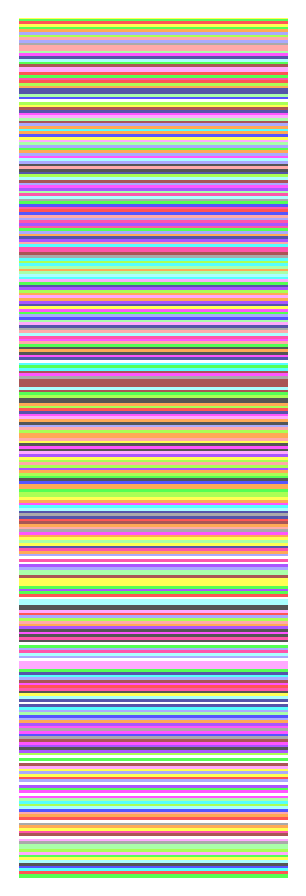
\includegraphics[width=0.14\textwidth]{resource/ground_truth.eps}
    }
    \subfigure[Random Noise]{
    \label{subfig:er_pdf}
    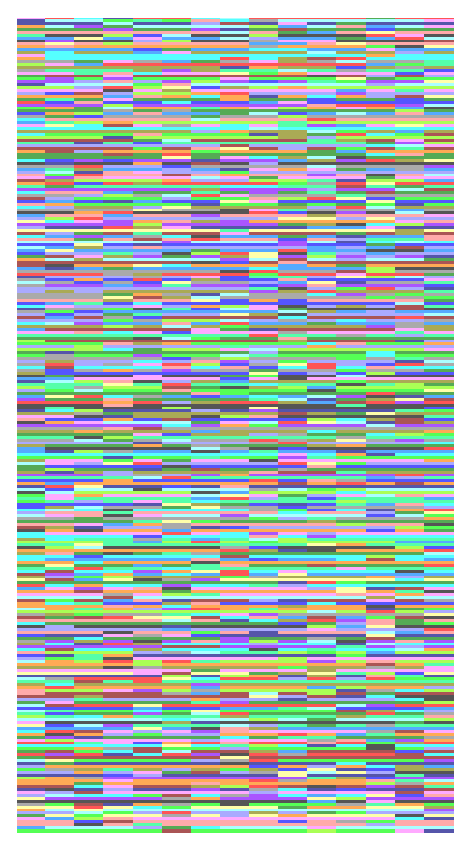
\includegraphics[width=0.14\textwidth]{resource/random_error.eps}
    }
    \subfigure[Our Recovered Result]{
    \label{subfig:re_pdf}
    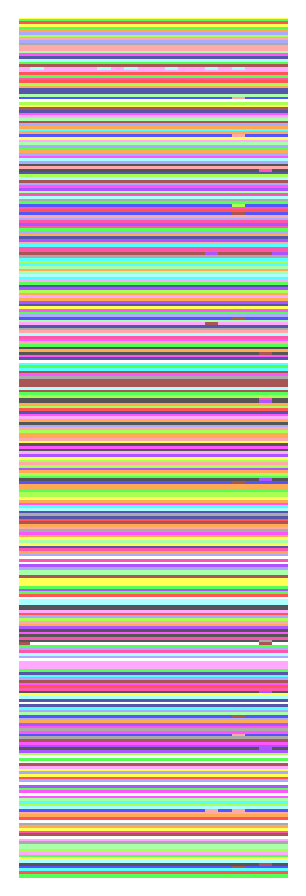
\includegraphics[width=0.14\textwidth]{resource/recover.eps}
    }
    \caption{Visualized results of the synthetic dataset.
    We use different colors to represent different label for each instance.
   Fig.~\ref{subfig:gt_pdf} show the visualized ground truth data,
   and each row corresponds to one instance with the class label represented by color.
   Fig.~\ref{subfig:er_pdf} has 15 columns, each represents one classifiers's predictions.
   There are also 15 columns in Fig.~\ref{subfig:re_pdf}, which is generated by the recovered results from our algorithm.
   %Each subfigure contains $n\times m$ small narrow blocks visualized in diverse color according to different labels.
    %Each picture represents a $280$ instances's information with every $20$ colums corresponding to one classifier.
    %We use different colors to represent different binary indicator predictions~(20 dimensions).
    %For~\ref{subfig:gt_pdf}, there is the ground truth information of $280$ instances for $15$ classifiers.
    %Obviously, the ground truth for different classifiers is the same.
    %Each kind of color represents one class, and the ground truth picture is generated from 280 synthetic instance lables.
    %Random noise picture~\ref{subfig:er_pdf} show 15 classifiers's prediction results while the classification accuracy for each one is about 60\%.
    %The last picture is the recovered result generated by our algorithm.
    Obviously, most of the outlier elements are correctly recovered by our algorithm with only a few error predictions left.
    }
    \label{fig:ensemble_cluster}
\end{figure}

As we can observe, our proposed algorithm significantly detect the outliers,
and furthermore, the outlier elements are accurately converted into the right predictions while preserving consistency among all classifiers.


%% Flower 17 Time [3.14] [229] [0.26] [1.62]


\subsection{Feature Extraction}
%We describe the details of the feature extraction for each dataset we use.
%All CNN features are extracted using Caffe~\cite{jia2014caffe}, a deep learning framework.
We used the best-performing CNN models for feature extraction including ResNet~\cite{he2015deep}, GoogleNet~\cite{szegedy2015going}, or etc.
These features are fairly state of the art.
They have been widely used in various recent research papers and have been verified the most effective features by recent internationally recognized competitions such as the ImageNet competition~\cite{russakovsky2015imagenet}.


In UCF101 dataset, five different features are extracted from the following:
%\begin{itemize}
%  \item `fc6' of C3D~\cite{tran2015learning}
%  \item `pool5/7x7\_s1' from GoogleNet~\cite{szegedy2015going}
%  \item `pool5' of ResNet-152~\cite{he2015deep}
%  \item two `fc6's of Two-Stream~\cite{simonyan2014two}
%\end{itemize}
`fc6' of C3D~\cite{tran2015learning},
`pool5/7x7\_s1' from GoogleNet~\cite{szegedy2015going},
`pool5' of ResNet-152~\cite{he2015deep},
and two `fc6's of Two-Stream~\cite{simonyan2014two}.
Given a video, we extract the above five features following the same process in~\cite{simonyan2014two,tran2015learning}(GoogleNet and ResNet-152 feature are same as spatial net in~\cite{simonyan2014two}).
All models we used are public available on Internet. %% provided by authors.

In Cifar10 dataset, the features are extracted from the `global\_pool' layer of ResNet-20,32,44,56,110~\cite{he2015deep} and of pre-activation ResNet-20,32,44,56,110,164 models~\cite{he2016identity}.
One feature is extracted from `pool3' layer's features of cifar10\_full model described in caffe example prototxt
\footnote{\url{https://github.com/BVLC/caffe/blob/master/examples/cifar10/cifar10_full.prototxt}}
.
Two modified networks VGG16 and GoogleNet are used to extract final pooling features~(Modify the stride 2 in conv4 and conv5 layers to stride 1 and fc layers to global pooling layers), trained the same in~\cite{he2015deep}
Each ResNet model is trained following the standard procedure in~\cite{he2015deep,he2016identity}, and cifar10\_full model is trained by an official shell
\footnote{\url{https://github.com/BVLC/caffe/blob/master/examples/cifar10/train_full.sh}}
before extracting features.
In Cifar100 dataset, we use `global\_pool' layer features of ResNet-20,32,44,56,68,110 and of pre-activation ResNet-20,32,44,56,110,164 models, following the same training process as in~\cite{he2015deep,he2016identity}.

In all other experiments, eight different features are extracted from the following:
%\begin{itemize}
%  \item `fc6' of VGG16,VGG19~\cite{chatfield2014return}
%  \item `fc6' of AlexNet,CaffeNet~\cite{krizhevsky2012imagenet}
%  \item `pool5/7x7\_s1' from GoogleNet~\cite{szegedy2015going}
%  \item `pool5' of ResNet-50,101,152~\cite{he2015deep}
%\end{itemize}
``fc6'' of VGG16, VGG19~\cite{chatfield2014return},
``fc6'' of AlexNet,CaffeNet~\cite{krizhevsky2012imagenet},
``pool5/7x7\_s1'' from GoogleNet~\cite{szegedy2015going},
and ``pool5'' of ResNet-50,101,152~\cite{he2015deep}.
We use the offical pre-trained model provided by Caffe Model Zoo
\footnote{\url{https://github.com/BVLC/caffe/wiki/Model-Zoo}}
.
For above eight models, we simply extract features with no extra operation.

\begin{table*}[t]
\centering
\begin{tabular}{c|c|c|c|c|c}
\hline
Method              & UCF-101          & CIFAR-10         & CIFAR-100        & Oxford-IIIT-Pet & PASCAL VOC 2007    \\\hline
ASF                 & 86.78\%          & 94.21\%          & 76.91\%          & 92.46\%         &   90.51\%          \\
MKL                 & 85.38\%          & 94.15\%          & 72.71\%          & 87.13\%         &   85.82\%          \\
RCEC                & 86.60\%          & 94.99\%          & 77.13\%          & 92.11\%         &   90.92\%          \\
FWOT                & -                & -                & -                & 92.90\%         &   91.20\%          \\
LPBoost             & 86.24\%          & 94.88\%          & 76.59\%          & 92.73\%         &   91.42\%          \\\hline
\textbf{Ours}       & \textbf{89.03\%} & \textbf{95.11\%} & \textbf{77.72\%} & \textbf{92.90\%}&   90.98\%          \\
\hline
\end{tabular}
\caption{Mean accuracy on real-world data sets.
FWOT costs excessive time for training UCF-101, CIFAR-10 , CIFAR-100~(over 24 hours),
so we omit these results indicated by ``-''.
}
\label{table:total_acc}
\end{table*}


\begin{table*}[t]
\centering
\begin{tabular}{c|c|c|c|c|c}
\hline
Method              & UCF-101    & CIFAR-10  & CIFAR-100  & Oxford-IIIT-Pet & PASCAL VOC 2007 \\\hline
RCEC                & 86.60      & 81.41     &  255.51    & 18.82           &   16.45         \\
FWOT                & $\infty$   & $\infty$  &  $\infty$  & 61697           &   19674         \\
LPBoost             & 110.81     & 72.45     &  4750.9    & 43.67           &   7.46          \\\hline
Ours                & 421.23     & 5.384     &  417.26    & 76.16           &   16.21         \\
\hline
\end{tabular}
\caption{Experimental results on real-world data sets. Computational time is recorded in seconds.
FWOT costs excessive time for training UCF-101, CIFAR-10 , CIFAR-100~(over 24 hours),
so we omit these results indicated by ``$\infty$''.}
\label{table:total_time}
\end{table*}



\subsection{Real-world Experiments}

In this section, we introduce the details about our experiments on each data set,
and demonstrate the empirical results in Table~\ref{table:total_acc} and Table~\ref{table:total_time}.
Five data sets are used to compare the performance on each contrast algorithm, including UCF-101, CIFAR-10, CIFAR-100, Oxford-III-Pet and PASCAL VOC 2007.
The computational cost of cross-validation is not counted in FWOT and LPBoost.

%\subsubsection{Experiment on UCF 101 dataset}
For action recognition, we present the comparison results on UCF 101 dataset.
UCF101 contains 13320 videos collected from YouTube, categoried into 101 human action classes.
We use the official split-1 described in~\cite{soomro2012ucf101}, which have 9573 training videos and 3783 testing videos.
As mentioned above, we extract fives features and train different classifier on each feature with the default parameters by liblinear.
Then by appling five classifiers on test data, we obtain $5 \times 101$ confidence scores for each video, which forms the input matrix $\bX$ of our algorithm.
Results are shown in Table~\ref{table:total_acc} and \ref{table:total_time}, in which we illustrate the performance of six fusion methods.
To be noted, FWOT is too slow to train, we do not show its result (more than one day).



%\subsubsection{Experiment on Cifar10 dataset}

In CIFAR-10 dataset, totally 60000 32x32 colour pictures are categoried into 10 classes, with 6000 pictures per class.
There are 50000 training data and 10000 testing data.
Fourteen CNN features are extracted from multiple state of the art models.
This experiments exhibit the ability of our algorithm to handle large scale data.

As we have 50000 training data and 10000 testing data,
FWOT algorithm has one step to deal with $n\times n$ matrixes, which are excessive to train~(more than one day).
LPBoost algorithm needs to create a $(n\calC - n) \times (1 + n + m)$ constraint matrix linear programming solvers
\footnote{\cite{gehler2009feature} use the MOSEK interior-point solver, see www.mosek.com.},
which occupies too much memory and still consumes long time to train,
so we solve this problem by using sparse matrices and parallel computation in MATLAB.
We also use `-s 2' parameters in liblinear to speedup training process.
Results of total six compared algorithms are shown in Table~\ref{table:total_acc} and \ref{table:total_time}.


%\subsubsection{Experiment on Cifar100 dataset}

CIFAR-100 is similar with CIFAR-10, except it has 100 classes containing 600 images each.
There are 50000 training data and 10000 testing data as CIFAR-10.
Twelve CNN features used in this experiment are described in the feature selection section.
Training and comparison process are the same as CIFAR-10.
Detailed results are shown in Table~\ref{table:total_acc} and \ref{table:total_time}.


%\subsubsection{Experiment on Oxford-IIIT-Pet dataset}

The Oxford-IIIT-Pet dataset contains 7349 images covering 37 different breeds of cats and dogs, 2371 images for cats and 4978 images for dogs.
There are roughly 200 pictures in each category with a large variations in multiple views, such as pose, scale and lighting.
We randomly sample fifty percent pictures as our training data and the others as testing data.
And then we train svm on each single feature and fuse the predictions by our proposed method.
We repeat the sample , training and fusion process five times to get fair results.
The comparison results are shown in Table~\ref{table:total_acc} and \ref{table:total_time}.

%% VOC07
PASCAL VOC 2007 is a dataset for object detection and image classification.
In our experiments, we only use the image level annotation information.
Since each image may contain more than one label, we filter the multi-label images to obtain 6146 clean data.
There is similar procesure of sampling, classification and fusion as in Oxford-IIIT-Pet.

From Table~\ref{table:total_acc}, our proposed algorithm provides significant improvement comparing with other effective late fusion methods on most datasets.
Addtionally, our algorithm is more efficient than other late fusion methods in most situations.
As we can see from Table~\ref{table:total_time}, some methods are not capable of handling large scale dataset.
However, ours can sovle the large scale problem efficiently.
%For example, the cost of FWOT is tremendous
%and it takes more than one day to fuse multiple results on CIFAR and UCF-101.
%With the growth of class number, LPBoost costs too much on data preparation affecting the overall efficiency.
%RCEC is usually faster than ours, but ours classification performance is better than its.

\subsection{Post Strategy Selection}

In this section, we compare three proposed post strategies on three small datasets: Wikipedia~\cite{rasiwasia2010new}, Oxford Flowers 17~\cite{nilsback2006visual} and Pascal Sentence~\cite{Li2006One}.
Wikipedia dataset contains paragraphs of text for each picture, and total 2866 image-text pairs are categoried into 10 class.
Only the image label annotation is used in our experiments.
PASCAL VOC 2007 contains 9963 images annotated with object-level information, which means each picture may have zero or more than one class.
We choose 6146 images classified into 20 classes by filtering out the no-single class data.
Oxford Flowers 17 has 17 flower categories with 80 images for each class.
Pascal Sentence contains 1000 images annotated by caption information and categoried into twenty classes.
Fifty percent of data are sampled as training set and the others as testing set, and experiments are repeated five times on above three datasets.

The $[$AVE$]$ strategy outperforms than the $[$VOTE$]$ in our experiments, which may be caused by the soft average method reserves more detail information than the hard voting method.
In all our experiments, the accuracy performance of the $[$GATE$]$ strategy is higher than the others.
Since the recover matrix $\bX$ contains the outlier rejection information,
it is more robust to take advantage of the recovered results as a confidence gate operating on the original confidence score matrix.

\begin{table}[ht]
\centering
\begin{tabular}{c|c|c|c}
\hline
Strategy            & Wikipedia         & Flowers 17          & Pascal Sentence     \\\hline
[AVE]               & 47.78\%           & \textbf{96.77\%}    & 66.40\%             \\\hline
[VOTE]              & 47.85\%           & 96.61\%             & 66.20\%             \\\hline
[GATE]              & \textbf{49.03\%}  & \textbf{96.77\%}    & \textbf{67.20\%}    \\
\hline
\end{tabular}
\caption{Mean accuracy using different strategies on three datasets.}
\label{table:strategy}
\end{table}

\subsection{Comparision with State-of-the-art}

In this sub-section, we compare the performance of our algorithm with the state-of-the-art techniques.
%we demonstrate experiments to compare the performance of our algorithm with the state-of-the-art techniques.
We use SVM classifiers based on different features in previous experiments to make a fair comparision with some MKL based mthods.
Since the performance of SVM classifiers usually are not as good as the results directly predicted by CNN models,
in order to obtain a higher result, we directly fuse multiple state-of-the-art CNN predictions.
Then we demonstrate the improvement of our fusion results compared to the state-of-the-art single model performance in Table.\ref{table:state_of_the_art}.

\begin{table}[ht]
\begin{center}
\begin{tabular}{ c | c | c }
    \hline
                                              & CIFAR-10             & CIFAR-100  \\\hline
\multirow{2}{*}{ResNet~\cite{he2016identity}} & 110, 134, 164        & 56, 110, 164  \\
                                              & $164^{*}$, $200^{*}$ & $110^{*}$, $164^{*}$  \\\hline
\multirow{2}{*}{WRN~\cite{zagoruyko2016wide}} & 16-10, 22-8, 28-10   & 16-10, 22-8, 28-10  \\
                                              &    40-4, 40-8        & 40-4  \\\hline
NIN~\cite{lin2013network}                     &     -                & -  \\ \hline
\end{tabular}
\end{center}
\caption{Model selection for CIFAR-10 dataset.
In the ResNet block, numbers repersent the depth of the selected models.
``*'' represents using the bottleneck block, otherwise using the basic block in residual networks.
In WRN block, ``x-y'', x represents the depth, and y represents the widening factor.
NIN network has only one formula, so we donot list its depth.}
\label{table:models}
\end{table}

\begin{table}[ht]
\centering
\begin{tabular}{c|c|c}\hline
                                                    &  CIFAR-10 & CIFAR-100  \\\hline
NIN~\cite{lin2013network}                           &   8.81    &  35.67     \\\hline
Highway~\cite{srivastava2015highway}                &   7.72    &  32.39     \\\hline
ELU~\cite{clevert2015fast}                          &   6.55    &  24.28     \\\hline
Pre-ResNet-1001~\cite{he2016identity}               &   4.92    &  22.71     \\\hline
WRN-28-10~\cite{zagoruyko2016wide}                  &   4.17    &  20.50     \\\hline
ResNeXt-29, $16\times64d$~\cite{xie2016aggregated}  &   3.58    &  17.31     \\\hline
Ours                                                &   3.47    &  17.24     \\\hline
\end{tabular}
\caption{Test error of different methods on CIFAR-10 and CIFAR-100 for different architectures.
}
\label{table:state_of_the_art}
\end{table}

We carefully cite the best performances reported in their papers
\cite{clevert2015fast,he2016identity,lin2013network,srivastava2015highway,xie2016aggregated,zagoruyko2016wide}
As we can observe, our fusion is capable of further improving the performance of single model by a large margin.
A single model has limited performance even with deeper depth or wider channel.
However, our fusion algorithm can achieve further improvement when the single model reaches the limit.
To be noticed, our method fuses multiple single models which all perform worse than ResNeXt~\cite{xie2016aggregated},
but can achieve low test error.
This demonstrates the benefit of a good late fusion method.

\section{Conclusion}

To relieve the performance degeneration in late label fusion from multiple sources, we formulate this problem as matrix factorization which recovers the underlying low-rank matrix and preserves the consistency among different sources.
%To deal with the dispute on combining multi-view predictions, we formulate the late fusion problem as a matrix recover problem.
%Our proposed algorithm is based on matrix factorization, which is unclear to consider smooth loss function from earlier research.
Existing matrix factorization algorithms usually consider smooth loss, while it is unclear how to extend them to handle nonsmooth robust loss, \eg, $\ell_{1,2}$ loss.
We propose an ALM based algorithm to solve matrix factorization problems with nonsmooth loss.
%Specifically, our proposed algorithm first rejects outliers on a label indicator matrix by $\ell_{1,2}$ loss,
%and then generates the predictions by combining robust outlier rejection information and prediction confidence scores from basic classifiers.
Empirical studies on large scale real-world data sets demonstrate that our proposed method can effectively improve performance compared to the state-of-the-art late fusion methods.

{\small
\bibliographystyle{ieee}
\bibliography{egbib}
}

\end{document}
